\section*{Questões}
\paragraph{1.}
\texttt{traceroute} antes do corte da ligação entre \textsf{R6} e \textsf{R7}:
\begin{verbatim}
R10#traceroute 172.16.1.2

Type escape sequence to abort.
Tracing the route to 172.16.1.2

  1 192.168.1.1 64 msec 60 msec 60 msec
  2 192.168.1.130 64 msec 60 msec 60 msec
  3 192.168.1.162 88 msec 96 msec 100 msec
  4 192.168.100.2 92 msec 88 msec 92 msec
  5 172.20.1.2 120 msec 120 msec 128 msec
  6 172.16.1.2 120 msec *  148 msec
\end{verbatim}\\
\texttt{traceroute} após o corte da ligação entre \textsf{R6} e \textsf{R7}:
\begin{verbatim}
R10#traceroute 172.16.1.2

Type escape sequence to abort.
Tracing the route to 172.16.1.2

  1 192.168.1.1 36 msec 32 msec 36 msec
  2 192.168.1.130 72 msec 60 msec 64 msec
  3 192.168.1.162 88 msec 92 msec 64 msec
  4 192.168.100.2 92 msec 88 msec 100 msec
  5  *  *  * 
  6  *  *  * 
  7  * 
    192.168.1.162 !H  * 
\end{verbatim}

\subparagraph{a.}
\begin{verbatim}
Router#show ip ospf database 

            OSPF Router with ID (0.0.0.6) (Process ID 6)

		Router Link States (Area 0)

Link ID         ADV Router      Age         Seq#       Checksum Link count
0.0.0.3         0.0.0.3         1670        0x80000003 0x00DDA3 1
0.0.0.4         0.0.0.4         1653        0x80000003 0x009DE6 1
0.0.0.5         0.0.0.5         1643        0x80000003 0x009BE5 1
0.0.0.6         0.0.0.6         1665        0x80000003 0x00B8C2 1

		Net Link States (Area 0)

Link ID         ADV Router      Age         Seq#       Checksum
192.168.100.2   0.0.0.6         1665        0x80000003 0x008EB9

		Summary Net Link States (Area 0)

Link ID         ADV Router      Age         Seq#       Checksum
172.16.2.0      0.0.0.6         1665        0x80000002 0x0090D2
172.17.0.0      0.0.0.6         1665        0x80000002 0x00FE5B
172.20.1.0      0.0.0.6         485         0x8000000A 0x00E480
172.20.1.8      0.0.0.6         1665        0x80000002 0x000952
172.20.1.12     0.0.0.6         1665        0x80000004 0x0078E6

		Router Link States (Area 1)

Link ID         ADV Router      Age         Seq#       Checksum Link count
0.0.0.6         0.0.0.6         496         0x80000006 0x006EE9 1
0.0.0.7         0.0.0.7         800         0x80000006 0x007F90 3
0.0.0.9         0.0.0.9         1599        0x80000003 0x005630 1

		Net Link States (Area 1)

Link ID         ADV Router      Age         Seq#       Checksum
172.20.1.2      0.0.0.7         796         0x80000004 0x00233F
172.20.1.6      0.0.0.9         1599        0x80000002 0x001546

		Summary Net Link States (Area 1)

Link ID         ADV Router      Age         Seq#       Checksum
172.16.2.0      0.0.0.6         1666        0x80000002 0x0090D2
172.17.0.0      0.0.0.6         1666        0x80000002 0x00FE5B
172.20.1.8      0.0.0.6         1666        0x80000002 0x000952
172.20.1.12     0.0.0.6         1666        0x80000004 0x0078E6
192.168.100.0   0.0.0.6         1666        0x80000004 0x00C19A
          
		Summary ASB Link States (Area 1)

Link ID         ADV Router      Age         Seq#       Checksum
0.0.0.3         0.0.0.6         1666        0x80000002 0x009B8C

		Router Link States (Area 2)

Link ID         ADV Router      Age         Seq#       Checksum Link count
0.0.0.6         0.0.0.6         1668        0x80000003 0x00403C 1
0.0.0.8         0.0.0.8         1603        0x80000004 0x000BE5 3
0.0.0.9         0.0.0.9         1600        0x80000003 0x006147 2

		Net Link States (Area 2)

Link ID         ADV Router      Age         Seq#       Checksum
172.20.1.9      0.0.0.9         1600        0x80000002 0x000552
172.20.1.13     0.0.0.8         1603        0x80000002 0x00BC9A

		Summary Net Link States (Area 2)

Link ID         ADV Router      Age         Seq#       Checksum
172.20.1.0      0.0.0.6         487         0x8000000A 0x00E480
192.168.100.0   0.0.0.6         1668        0x80000004 0x00C19A

		Summary ASB Link States (Area 2)

Link ID         ADV Router      Age         Seq#       Checksum
0.0.0.3         0.0.0.6         1668        0x80000002 0x009B8C

		Type-5 AS External Link States

Link ID         ADV Router      Age         Seq#       Checksum Tag
192.168.1.0     0.0.0.3         1673        0x80000002 0x003D24 0
192.168.1.128   0.0.0.3         1673        0x80000002 0x007A06 0
192.168.1.160   0.0.0.3         1673        0x80000002 0x003927 0
192.168.1.192   0.0.0.3         1673        0x80000002 0x00F748 0
192.168.1.224   0.0.0.3         1673        0x80000002 0x00B669 0
\end{verbatim}

\subparagraph{b.}
O corte da ligação entre \textsf{R6} e \textsf{R7} não fez com que o percurso dos pacotes fosse desviado de modo a atravessar \textsf{R8} e \textsf{R9}, uma vez que, como podemos verificar no \texttt{show ip ospf database} obtido na alínea anterior, o \emph{router} \textsf{R6} "conhece" todos os \emph{routers} envolvidos e em especial o \textsf{R7}, (\texttt{Router Link States (Area 1)}), para a qual tem uma rota intra-área que é sempre preferida pelo OSPF.

\paragraph{2.}
\subparagraph{a.}
Como podemos verificar a baixo, no \emph{router} \textsf{R8}, o estado do vizinho \textsf{R9} fica \texttt{DOWN}, (\texttt{state DOWN}). O evento que ocorreu nesse instante e despoletou essa mudança foi o IE2 (ver lista dos eventos de transição na tabela 8-1 do livro Routing TCP/IP, vol.1, 2ª ed).

\begin{verbatim}
Router#debug ip ospf adj 
OSPF adjacency events debugging is on
Router#
*Apr 14 15:58:38.411: OSPF: 0.0.0.9 address 172.20.1.9 on FastEthernet1/1 is dead
*Apr 14 15:58:38.411: OSPF: 0.0.0.9 address 172.20.1.9 on FastEthernet1/1 is dead,
 state DOWN
*Apr 14 15:58:38.411: %OSPF-5-ADJCHG: Process 8, Nbr 0.0.0.9 on FastEthernet1/1 
from FULL to DOWN, Neighbor Down: Dead timer expired
*Apr 14 15:58:38.415: OSPF: Neighbor change Event on interface FastEthernet1/1
*Apr 14 15:58:38.415: OSPF: DR/BDR election on FastEthernet1/1 
*Apr 14 15:58:38.415: OSPF: Elect BDR 0.0.0.8
*Apr 14 15:58:38.415: OSPF: Elect DR 0.0.0.8
*Apr 14 15:58:38.415: OSPF: Elect BDR 0.0.0.0
*Apr 14 15:58:38.415: OSPF: Elect DR 0.0.0.8
*Apr 14 15:58:38.419:        DR: 0.0.0.8 (Id)   BDR: none 
*Apr 14 15:58:38.419: OSPF: Remember old DR 0.0.0.9 (id)
*Apr 14 15:58:38.915: OSPF: Build router LSA for area 2, router ID 0.0.0.8, 
 seq 0x80000005
*Apr 14 15:58:38.919: OSPF: No full nbrs to build Net Lsa for interface 
 FastEthernet1/1
\end{verbatim}

\newpage

\subparagraph{b.}
\textsf{R8} envia um \emph{LS Update} para a rede \emph{multicast} 224.0.0.5 no instante em que deteta que \textsf{R9} "morreu", nesta mensagem é enviado um LSA (\texttt{Router-LSA}).
O objetivo dos LAS's é permitir construir um grafo dirigido da rede para posteriormente se calcular o caminho mais curto para cada destino.\\
O \emph{Router LSA}, enviado por \textsf{R8}, serve para este se anunciar e identificar as suas ligações na área a que pertence juntamente com as respetivas métricas, de forma a se poder cumprir com o objetivos dos LSA's. Uma vez que \textsf{R8} deteta que um vizinho, \textsf{R9}, "morreu" este envia um \emph{Router LSA} para se poder "construir" um novo grafo dirigido com a atualização das suas ligações. \textsf{R8} informa então que tem 3 ligações disponíveis ,\texttt{Number of Links=3}, em que uma é de trânsito, \texttt{Type: Transit}, (informando que o endereço IP do \emph{Designated Router} é 172.20.1.13, o próprio \textsf{R8}, e a métrica é 10), e as duas ligações restantes são \emph{stub} (ponta), \textsf{Type: stub}, em que uma tem número de IP da rede/subrede 172.20.1.8 com métrica 10 e a outra tem número de IP da rede/subrede 172.16.2.0 com métrica 10 .

\begin{figure}[h]
\centering
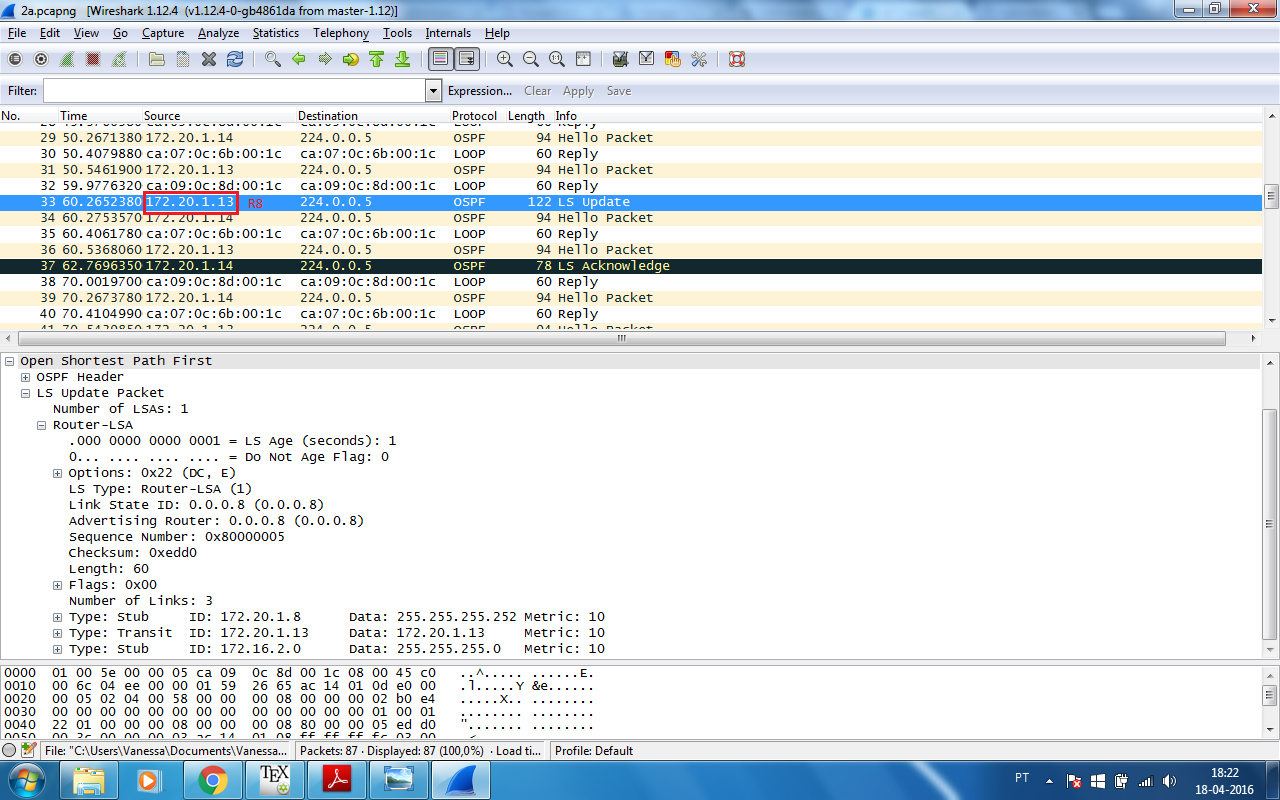
\includegraphics[width=1\textwidth, height=0.45\textheight]{2b.png}
\label{fig:captura R8-R6}
\caption{Captura de pacotes na ligação entre \textsf{R6} e \textsf{R8}.}
\end{figure}

\subparagraph{c.}
A mensagem que permite ao \emph{router} \textsf{R9} saber que tem comunicação bidirecional (\emph{two-way}) com \textsf{R8} apresenta-se na figura 3, devidamente sinalizada. Escolhemos esta mensagem, \emph{Hello Packet}, uma vez que é o sub-protocolo \emph{Hello} que verifica conexões bidirecionais entre os vizinhos. Quando um \emph{router}, \textsf{R8}, deteta o seu \emph{Router ID} num \emph{Hello} recebido, sabe que existe comunicação bidirecional com o vizinho que o enviou, \textsf{R9}, como se pode analisar na figura.

\begin{figure}[h]
\centering
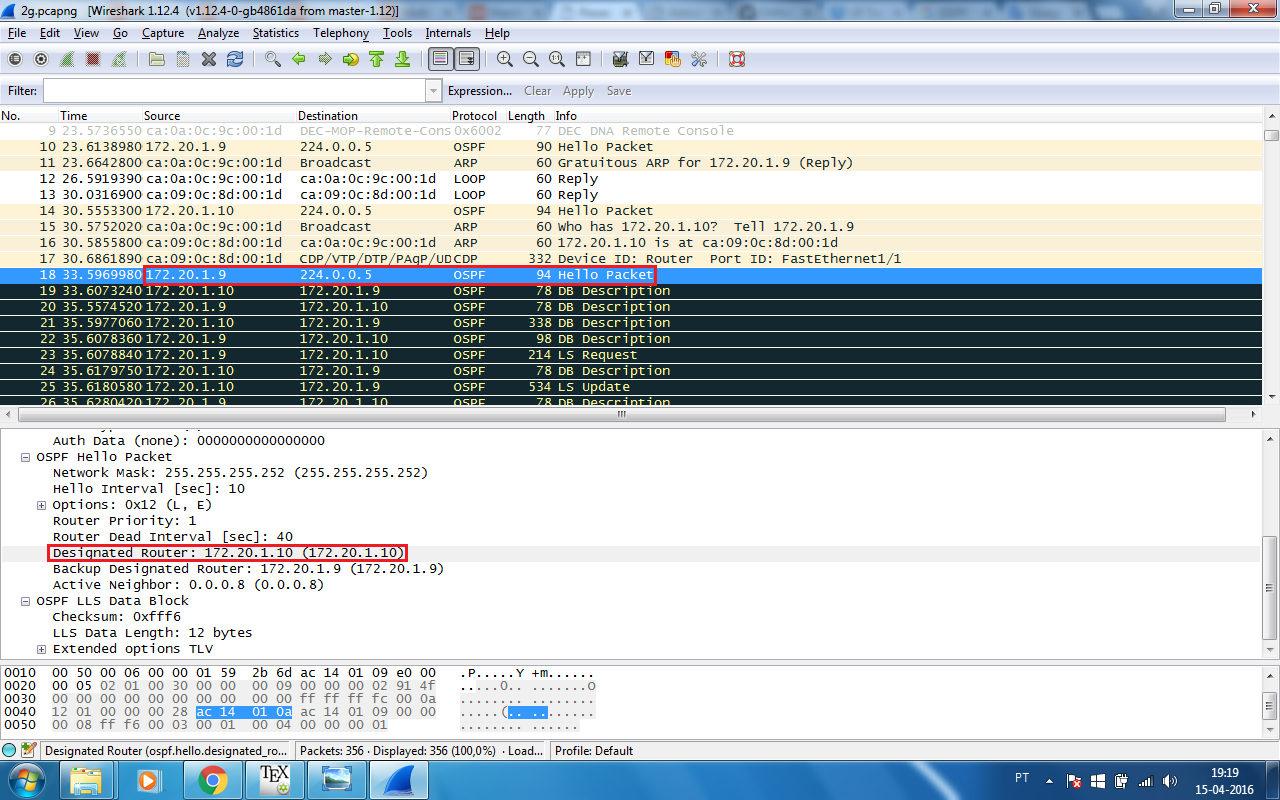
\includegraphics[width=1\textwidth, height=0.45\textheight]{2c.png}
\label{fig:captura R8-R9}
\caption{Captura de pacotes na ligação entre \textsf{R8} e \textsf{R9}.}
\end{figure}

\newpage

\subparagraph{d.}

No ficheiro que contem a captura de \textsf{R8-R9} (Capturas Wireshark/2g.pcapng) encontramos vários
tipos de anúncios em cada mensagem \emph{LS Update}:
\begin{itemize}
  \item Tipo 1 - Router LSA - no pacote 25, servindo para o \emph{router} \textsf{R8}
    identificar e partilhar as suas ligações.
  \item Tipo 2 - Network LSA - servindo para o \emph{router} designado informar
    sobre os \emph{routers} ligado ao nó virtual correspondente à rede
    do DR.
  \item Tipo 3 - Network Summary - informa sobre os destinos
    sumarizados com custos a partir do Area Border Router, neste caso
    o R3.
  \item Tipo 4 - ASBR Summary - Rota para o \emph{router Autonomous System Boundary
    Router} que gerou os LSAs de tipo 5.
  \item Tipo 5 - AS External LSA - servindo para o \emph{router}
    informar sobre os destinos externos ao OSPF. Neste caso em
    particular, as rotas externas são todas do Tipo 2 pois são
    importadas de uma métrica incompatível com OSPF.
\end{itemize}

\subparagraph{e.} Campos Link State ID:
\begin{itemize}
\item Tipo 1 - ID do router que gerou o LSA.
\item Tipo 2 - Endereço IP da interface do DR nessa rede.
\item Tipo 3 - Endereço IP da rede de destino.
\item Tipo 4 - Router ID do ASBR que gerou o AS External LSA.
\item Tipo 5 - Endereço IP da rede de destino do External LSA.
\end{itemize}
Advertising Router - ID do \emph{router} que gera o LSA.
Nos LSA do tipo 1, dentro de cada entrada LSA (LinkID, LinkData,
LinkType, Metric), podemos construir um grafo com adjacência entre
destinos e o \emph{router} que emite o LSA. Exemplo (pacote 25, \emph{advertising
router} 0.0.0.8):
\begin{verbatim}
Type: Stub     ID: 172.20.1.8      Data: 255.255.255.252 Metric: 10
    Link ID: 172.20.1.8 - IP network/subnet number
    Link Data: 255.255.255.252
    Link Type: 3 - Connection to a stub network
    Number of Metrics: 0 - TOS
    0 Metric: 10
\end{verbatim}
Nos LSA do tipo 2, a informação em ``Attached router'' permite separar
o grafo nas suas componentes fortemente conexas, separando-o em
``áreas'':
\begin{verbatim}
LSA-type 2 (Network-LSA), len 32
    .000 0000 1101 1101 = LS Age (seconds): 221
    0... .... .... .... = Do Not Age Flag: 0
    Options: 0x22 ((DC) Demand Circuits, (E) External Routing)
    LS Type: Network-LSA (2)
    Link State ID: 172.20.1.13
    Advertising Router: 0.0.0.8
    Sequence Number: 0x80000003
    Checksum: 0xba9b
    Length: 32
    Netmask: 255.255.255.252
    Attached Router: 0.0.0.8
    Attached Router: 0.0.0.6
\end{verbatim}
Nos LSA do tipo 5, podemos acrescentar ao grafo informação sobre os
destinos externos ao OSPF e a sua adjacência ao ASBR:
\begin{verbatim}
LSA-type 5 (AS-External-LSA (ASBR)), len 36
    .000 0000 1111 0101 = LS Age (seconds): 245
    0... .... .... .... = Do Not Age Flag: 0
    Options: 0x20 ((DC) Demand Circuits)
    LS Type: AS-External-LSA (ASBR) (5)
    Link State ID: 192.168.1.224
    Advertising Router: 0.0.0.3
    Sequence Number: 0x80000003
    Checksum: 0xb46a
    Length: 36
    Netmask: 255.255.255.224
    1... .... = External Type: Type 2 (metric is larger than any other link state path)
    .000 0000 = TOS: 0
    Metric: 100
    Forwarding Address: 0.0.0.0
    External Route Tag: 0
\end{verbatim}

\subparagraph{f.}

O último anúncio do tipo \emph{Router LSA} originado pelo \emph{router} \textsf{R8} é o pacote 1761, do ficheiro Capturas Wireshark/2g.pcapng, que se apresenta a seguir e onde podemos ver, para cada uma das ligações, o respetivo tipo, campos ID e Data e os seus significados:
\begin{verbatim}
LSA-type 1 (Router-LSA), len 60
    .000 0000 0000 0101 = LS Age (seconds): 5
    0... .... .... .... = Do Not Age Flag: 0
    Options: 0x22 ((DC) Demand Circuits, (E) External Routing)
    LS Type: Router-LSA (1)
    Link State ID: 0.0.0.8
    Advertising Router: 0.0.0.8
    Sequence Number: 0x80000003
    Checksum: 0x0de4
    Length: 60
    Flags: 0x00
    Number of Links: 3
    Type: Transit  ID: 172.20.1.9      Data: 172.20.1.10     Metric: 10
        Link ID: 172.20.1.9 - IP address of Designated Router
        Link Data: 172.20.1.10 - endereço IP do router nessa rede
        Link Type: 2 - Connection to a transit network
        Number of Metrics: 0 - TOS
        0 Metric: 10
    Type: Transit  ID: 172.20.1.13     Data: 172.20.1.13     Metric: 10
        Link ID: 172.20.1.13 - IP address of Designated Router
        Link Data: 172.20.1.13 - endereço IP do router nessa rede
        Link Type: 2 - Connection to a transit network
        Number of Metrics: 0 - TOS
        0 Metric: 10
    Type: Stub     ID: 172.16.2.0      Data: 255.255.255.0   Metric: 10
        Link ID: 172.16.2.0 - IP network/subnet number (prefixo)
        Link Data: 255.255.255.0 - máscara da rede
        Link Type: 3 - Connection to a stub network
        Number of Metrics: 0 - TOS
        0 Metric: 10
\end{verbatim}

\subparagraph{g.}
Pacote 1737: \textsf{R8} a \textsf{R9}.
\begin{verbatim}
LSA-type 1 (Router-LSA), len 60
    .000 0000 0010 1011 = LS Age (seconds): 43
    0... .... .... .... = Do Not Age Flag: 0
    Options: 0x22 ((DC) Demand Circuits, (E) External Routing)
    LS Type: Router-LSA (1)
    Link State ID: 0.0.0.8
    Advertising Router: 0.0.0.8
    Sequence Number: 0x80000001
    Checksum: 0xdab9
    Length: 60
    Flags: 0x00
    Number of Links: 3
    Type: Stub     ID: 172.20.1.8      Data: 255.255.255.252 Metric: 10
        Link ID: 172.20.1.8 - IP network/subnet number
        Link Data: 255.255.255.252
        Link Type: 3 - Connection to a stub network
        Number of Metrics: 0 - TOS
        0 Metric: 10
    Type: Stub     ID: 172.20.1.12     Data: 255.255.255.252 Metric: 10
        Link ID: 172.20.1.12 - IP network/subnet number
        Link Data: 255.255.255.252
        Link Type: 3 - Connection to a stub network
        Number of Metrics: 0 - TOS
        0 Metric: 10
    Type: Stub     ID: 172.16.2.0      Data: 255.255.255.0   Metric: 10
        Link ID: 172.16.2.0 - IP network/subnet number
        Link Data: 255.255.255.0
        Link Type: 3 - Connection to a stub network
        Number of Metrics: 0 - TOS
        0 Metric: 10
\end{verbatim}

Após um \emph{Hello Packet} (cujo propósito é estabelecer conexões bidirecionais) de \textsf{R9}, o \emph{router} \textsf{R8} responde com uma \emph{BD Description} cujo propósito é descrever as ligações entre cada \emph{router} com os seus parceiros adjacentes. Seguidamente há um \emph{LS   Request} de \textsf{R9} para \textsf{R10}, \texttt{terminal 1}, pedindo informação desta forma. Como resposta a este pedido o \textsf{R10} envia um \emph{LS Update}. Cada LSA é finalmente confirmado com um \emph{LS Acknowledge} por cada recetor.

\paragraph{3.}
\emph{Router} \textsf{R3}:
\begin{verbatim}
Router#show ip ospf interface FastEthernet 1/1
%OSPF: OSPF not enabled on FastEthernet1/1
Router#show ip ospf interface FastEthernet 1/0
%OSPF: OSPF not enabled on FastEthernet1/0
Router#show ip ospf interface FastEthernet 2/0
FastEthernet2/0 is up, line protocol is up 
  Internet Address 192.168.100.1/24, Area 0 
  Process ID 3, Router ID 0.0.0.3, Network Type BROADCAST, Cost: 10
  Transmit Delay is 1 sec, State DROTHER, Priority 1 
  Designated Router (ID) 0.0.0.6, Interface address 192.168.100.2
  Backup Designated router (ID) 0.0.0.5, Interface address 192.168.100.254
  Timer intervals configured, Hello 10, Dead 40, Wait 40, Retransmit 5
    oob-resync timeout 40
    Hello due in 00:00:00
  Supports Link-local Signaling (LLS)
  Index 1/1, flood queue length 0
  Next 0x0(0)/0x0(0)
  Last flood scan length is 0, maximum is 5
  Last flood scan time is 0 msec, maximum is 4 msec
  Neighbor Count is 3, Adjacent neighbor count is 2 
    Adjacent with neighbor 0.0.0.5  (Backup Designated Router)
    Adjacent with neighbor 0.0.0.6  (Designated Router)
  Suppress hello for 0 neighbor(s)
\end{verbatim}

\emph{Router} \textsf{R4}:
\begin{verbatim}
Router#show ip ospf interface FastEthernet 1/0
FastEthernet1/0 is up, line protocol is up 
  Internet Address 192.168.100.253/24, Area 0 
  Process ID 4, Router ID 0.0.0.4, Network Type BROADCAST, Cost: 10
  Transmit Delay is 1 sec, State DROTHER, Priority 1 
  Designated Router (ID) 0.0.0.6, Interface address 192.168.100.2
  Backup Designated router (ID) 0.0.0.5, Interface address 192.168.100.254
  Timer intervals configured, Hello 10, Dead 40, Wait 40, Retransmit 5
    oob-resync timeout 40
    Hello due in 00:00:08
  Supports Link-local Signaling (LLS)
  Index 1/1, flood queue length 0
  Next 0x0(0)/0x0(0)
  Last flood scan length is 0, maximum is 1
  Last flood scan time is 0 msec, maximum is 4 msec
  Neighbor Count is 3, Adjacent neighbor count is 2 
    Adjacent with neighbor 0.0.0.5  (Backup Designated Router)
    Adjacent with neighbor 0.0.0.6  (Designated Router)
  Suppress hello for 0 neighbor(s)
\end{verbatim}

\emph{Router} \textsf{R5}:
\begin{verbatim}
Router#show ip ospf interface FastEthernet 1/0
FastEthernet1/0 is up, line protocol is up 
  Internet Address 192.168.100.254/24, Area 0 
  Process ID 5, Router ID 0.0.0.5, Network Type BROADCAST, Cost: 10
  Transmit Delay is 1 sec, State BDR, Priority 1 
  Designated Router (ID) 0.0.0.6, Interface address 192.168.100.2
  Backup Designated router (ID) 0.0.0.5, Interface address 192.168.100.254
  Timer intervals configured, Hello 10, Dead 40, Wait 40, Retransmit 5
    oob-resync timeout 40
    Hello due in 00:00:01
  Supports Link-local Signaling (LLS)
  Index 1/1, flood queue length 0
  Next 0x0(0)/0x0(0)
  Last flood scan length is 0, maximum is 1
  Last flood scan time is 0 msec, maximum is 4 msec
  Neighbor Count is 3, Adjacent neighbor count is 3 
    Adjacent with neighbor 0.0.0.3
    Adjacent with neighbor 0.0.0.4
    Adjacent with neighbor 0.0.0.6  (Designated Router)
  Suppress hello for 0 neighbor(s)
\end{verbatim}

\emph{Router} \textsf{R6}:
\begin{verbatim}
Router#show ip ospf interface FastEthernet 1/0
FastEthernet1/0 is up, line protocol is up 
  Internet Address 172.20.1.14/30, Area 2 
  Process ID 6, Router ID 0.0.0.6, Network Type BROADCAST, Cost: 10
  Transmit Delay is 1 sec, State BDR, Priority 1 
  Designated Router (ID) 0.0.0.8, Interface address 172.20.1.13
  Backup Designated router (ID) 0.0.0.6, Interface address 172.20.1.14
  Timer intervals configured, Hello 10, Dead 40, Wait 40, Retransmit 5
    oob-resync timeout 40
    Hello due in 00:00:04
  Supports Link-local Signaling (LLS)
  Index 1/2, flood queue length 0
  Next 0x0(0)/0x0(0)
  Last flood scan length is 1, maximum is 6
  Last flood scan time is 0 msec, maximum is 4 msec
  Neighbor Count is 1, Adjacent neighbor count is 1 
    Adjacent with neighbor 0.0.0.8  (Designated Router)
  Suppress hello for 0 neighbor(s)
Router#show ip ospf interface FastEthernet 1/1
FastEthernet1/1 is up, line protocol is up 
  Internet Address 172.20.1.1/30, Area 1 
  Process ID 6, Router ID 0.0.0.6, Network Type BROADCAST, Cost: 10
  Transmit Delay is 1 sec, State DR, Priority 1 
  Designated Router (ID) 0.0.0.6, Interface address 172.20.1.1
  Backup Designated router (ID) 0.0.0.7, Interface address 172.20.1.2
  Timer intervals configured, Hello 10, Dead 40, Wait 40, Retransmit 5
    oob-resync timeout 40
    Hello due in 00:00:02
  Supports Link-local Signaling (LLS)
  Index 1/1, flood queue length 0
  Next 0x0(0)/0x0(0)
  Last flood scan length is 1, maximum is 6
  Last flood scan time is 0 msec, maximum is 4 msec
  Neighbor Count is 1, Adjacent neighbor count is 1 
    Adjacent with neighbor 0.0.0.7  (Backup Designated Router)
  Suppress hello for 0 neighbor(s)
Router#show ip ospf interface FastEthernet 2/0
FastEthernet2/0 is up, line protocol is up 
  Internet Address 192.168.100.2/24, Area 0 
  Process ID 6, Router ID 0.0.0.6, Network Type BROADCAST, Cost: 10
  Transmit Delay is 1 sec, State DR, Priority 1 
  Designated Router (ID) 0.0.0.6, Interface address 192.168.100.2
  Backup Designated router (ID) 0.0.0.5, Interface address 192.168.100.254
  Timer intervals configured, Hello 10, Dead 40, Wait 40, Retransmit 5
    oob-resync timeout 40
    Hello due in 00:00:00
  Supports Link-local Signaling (LLS)
  Index 1/3, flood queue length 0
  Next 0x0(0)/0x0(0)
  Last flood scan length is 1, maximum is 8
  Last flood scan time is 0 msec, maximum is 4 msec
  Neighbor Count is 3, Adjacent neighbor count is 3 
    Adjacent with neighbor 0.0.0.3
    Adjacent with neighbor 0.0.0.4
    Adjacent with neighbor 0.0.0.5  (Backup Designated Router)
  Suppress hello for 0 neighbor(s)
\end{verbatim}

\subparagraph{a.}
O \emph{router} \textsf{R3} contêm 2 adjacências, na \texttt{interface FastEthernet 2/0}.\\
O \emph{router} \textsf{R4} contêm 2 adjacências, na \texttt{interface FastEthernet 1/0}.\\
O \emph{router} \textsf{R5} contêm 3 adjacências, na \texttt{interface FastEthernet 1/0}.\\
O \emph{router} \textsf{R6} contêm 1 adjacências, na \texttt{interface FastEthernet 1/0}, 1 adjacências, na \texttt{interface FastEthernet 1/1} e 3 adjacências, na \texttt{interface FastEthernet 2/0}, tendo assim um total de 5 adjacências.\\
\textsf{R6} é o \emph{Designated Router} e por isso, não é de estranhar que seja o \emph{router} com maior número de adjacências, isto implicaria um grande volume de troca de informações de encaminhamento.\\
\textsf{R5} é o segundo \emph{router} com maior número de adjacências e por isso é o \emph{Backup Designated Router}, que tem o papel de toma o lugar do \emph{Designated Router} caso ele falhe.\\
Já \textsf{R3} e \textsf{R4} são \emph{DROthers} que estabelecem adjacências apenas com o \emph{Designated Router}, \textsf{R6}, e com o \emph{Backup Designated Router}, \textsf{R5}.

\subparagraph{b.}
No OSPF o \emph{Designated Router} serve para gerir o processo de inundação na rede de acesso múltiplo e gerar informação topológica sobre um nó virtual que representa a rede de acesso múltiplo.

\paragraph{4.}
\subparagraph{a.}
O caminho seguido pelos pacotes ICMP \emph{echo request} é do IP 172.16.1.2, \textbf{\texttt{Terminal 2}}, passando por \textbf{\textsf{R7}}, de seguida por \textbf{\textsf{R6}} e por \textbf{\textsf{R8}} chegando ao destino, interface 172.17.0.1 de \textsf{R9}.\\
O caminho seguido pelos pacotes ICMP \emph{echo reply} é da interface 172.17.0.1 de \textbf{\textsf{R9}} passando por \textbf{\textsf{R7}} e por último chega ao destino, \textbf{\textsf{Terminal 2}}.\\
Os pacotes ICMP seguem caminhos diferentes por causa das rotas especificadas pelo protocolo OSPF para cada \emph{router}. O \emph{router} \textsf{R7} tem rota definida para \textsf{R9} através de \textsf{R6}, (\texttt{O IA 172.17.0.0/16 [110/40] via 172.20.1.1, 00:16:38, FastEthernet1/0}), enquanto que o \emph{router} \textsf{R9} tem a rota para \textsf{Terminal 2} através de \textsf{R7}, (\texttt{O 172.16.1.0 [110/20] via 172.20.1.5, 00:17:29, FastEthernet1/0}).

\begin{figure}[h]
\centering
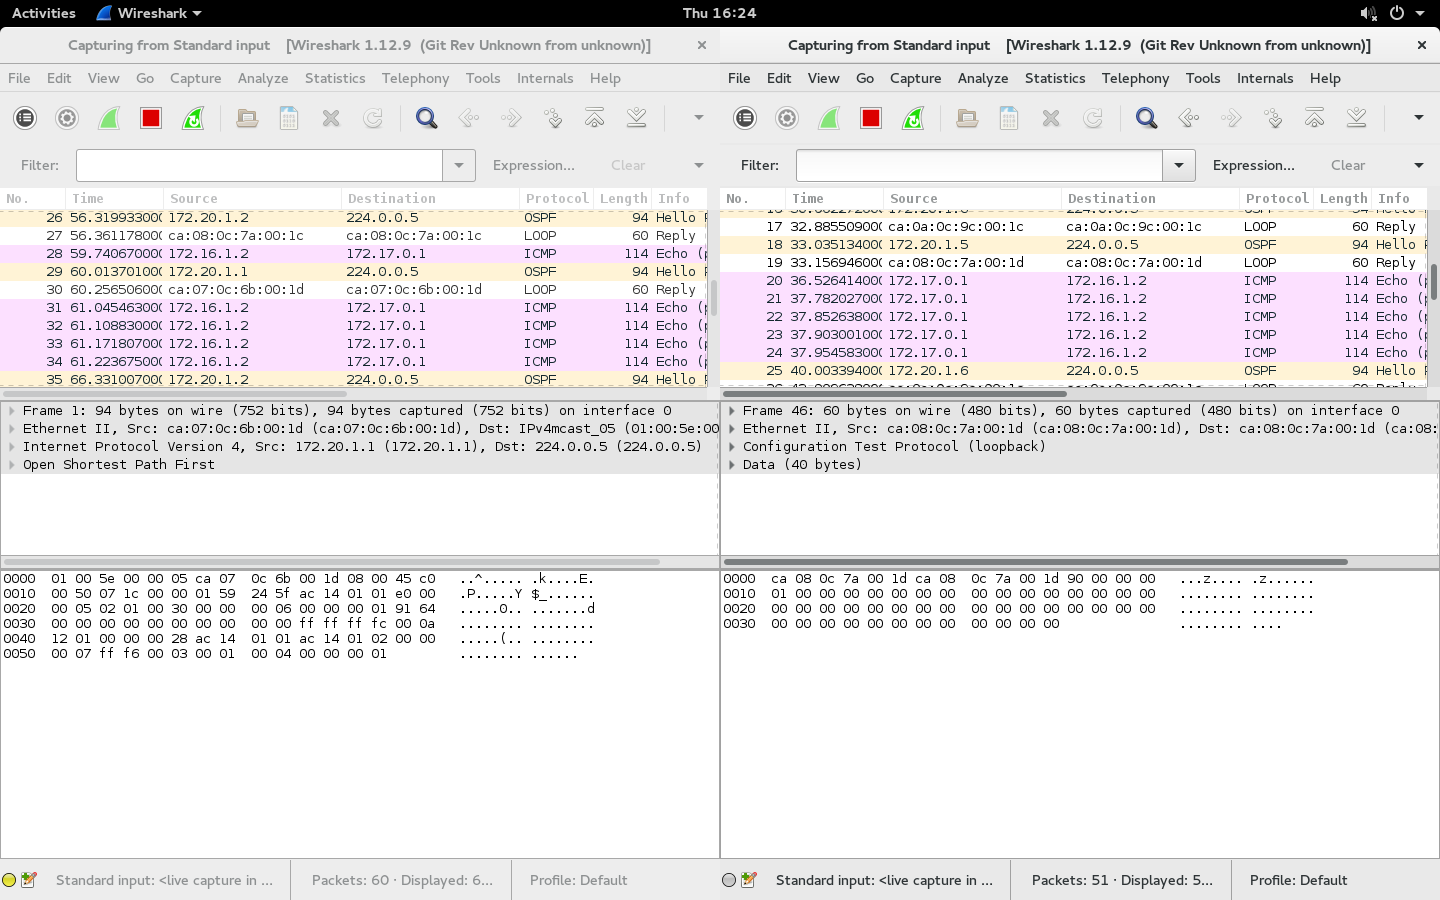
\includegraphics[width=1\textwidth, height=0.35\textheight]{4a.png}
\label{fig:captura R7}
\caption{Captura de pacotes na ligação entre as interfaces 172.20.1.2 e 172.20.1.5 de \textsf{R7}.}
\end{figure}

\subparagraph{b.}
Nós tentamos alterar o custo da interface 172.20.1.6 para um valor elevado, (\texttt{ip ospf cost 65000}), para tentar que a ligação se corrompa, de modo a que o percurso do \emph{echo reply} seja o inverso do do \emph{echo request}. Tentamos ainda para o valor máxima, (\texttt{ip ospf cost 65535}), mas não obtemos sucesso.\\
O percurso não foi alterado pois os \emph{routers} internos de cada área têm penas uma base de dados topológica dessa área. O \emph{router} \textsf{R6} é um \emph{Area Border Router} logo, conhece a topologia das áreas às quais está ligado, área 1 e 2. Deste modo, uma vez que o \textsf{Terminal 2} só pertence à área 1, o melhor caminho continua a ser por essa área, e não passando por outra área, área 2.

\begin{figure}[h]
\centering
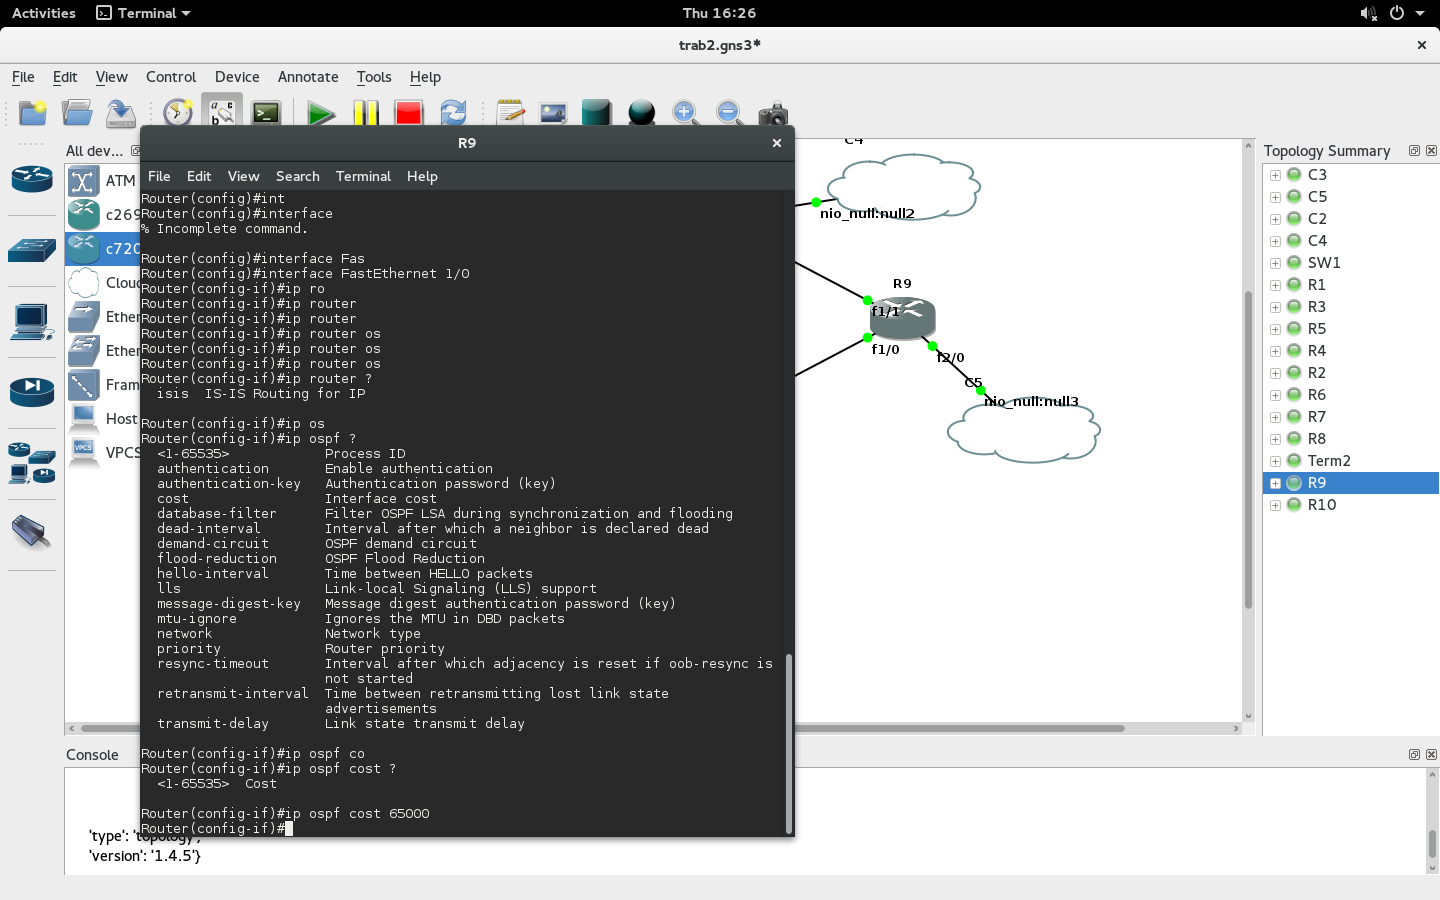
\includegraphics[width=1\textwidth, height=0.25\textheight]{4b.png}
\label{fig:custo da interface}
\caption{Alteração do custo da interface 172.20.1.6 de \textsf{R9}.}
\end{figure}

\begin{figure}[h]
\centering
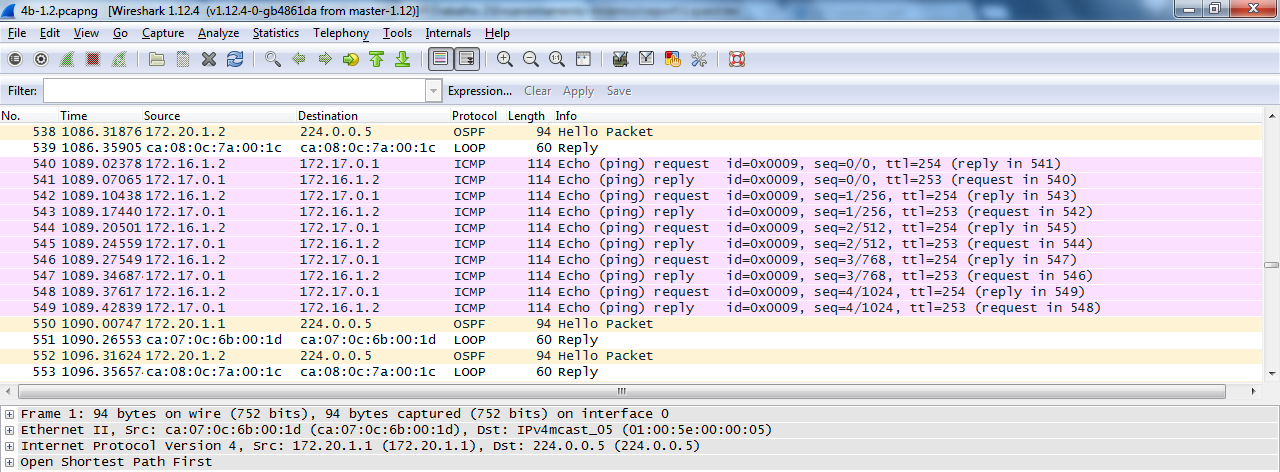
\includegraphics[width=1\textwidth, height=0.25\textheight]{4b_.png}
\label{fig:captura}
\caption{Captura de pacotes na ligação entre as interfaces 172.20.1.2 e 172.20.1.5 de \textsf{R7}.}
\end{figure}

\paragraph{5.}
Como podemos verificar na figura 7, as mensagens RIP trocadas entre \textsf{R1} e \textsf{R2} são inicialmente enviadas para o IP 255.255.255.255, uma vez que o \emph{broadcast} estava ativado. Uma vez desativado as mensagens RIP são enviadas para o IP 224.0.0.9.\\
Os \emph{routers} RIP foram configurados de modo a correrem a versão 2 do protocolo, e por isso as mensagens são enviadas para o IP 224.0.0.9, que é um endereço \emph{multicast} "todos os \emph{routers} RIPv2".
Isto evita que os terminais recebam os anúncios, que não lhes interessam.

\newpage

\begin{figure}[h]
\centering
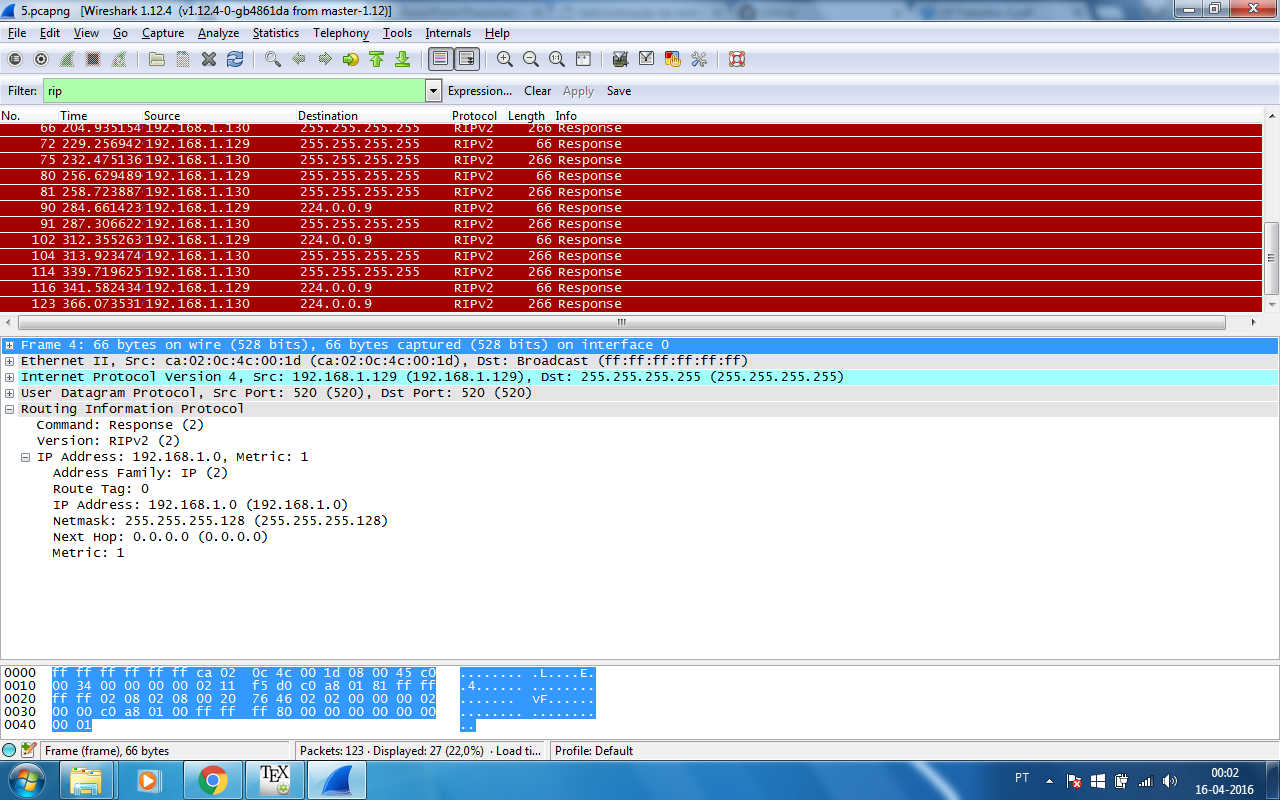
\includegraphics[width=1\textwidth, height=0.45\textheight]{5.png}
\label{fig:captura}
\caption{Capture de mensagens RIP trocadas entre \textsf{R1} e \textsf{R2}.}
\end{figure}

\paragraph{6.}
\begin{verbatim}
*Apr 14 17:00:31.055: RIP: sending v2 update to 224.0.0.9 via
 FastEthernet1/1 (192.168.1.130)
*Apr 14 17:00:31.055: RIP: build update entries
*Apr 14 17:00:31.055: 	172.16.1.0/24 via 0.0.0.0, metric 6, tag 0
*Apr 14 17:00:31.059: 	172.16.2.0/24 via 0.0.0.0, metric 6, tag 0
*Apr 14 17:00:31.059: 	172.17.0.0/16 via 0.0.0.0, metric 6, tag 0
*Apr 14 17:00:31.059: 	172.20.1.0/30 via 0.0.0.0, metric 6, tag 0
*Apr 14 17:00:31.059: 	172.20.1.4/30 via 0.0.0.0, metric 6, tag 0
*Apr 14 17:00:31.063: 	172.20.1.8/30 via 0.0.0.0, metric 6, tag 0
*Apr 14 17:00:31.063: 	172.20.1.12/30 via 0.0.0.0, metric 6, tag 0
*Apr 14 17:00:31.063: 	192.168.1.160/27 via 0.0.0.0, metric 1, tag 0
*Apr 14 17:00:31.067: 	192.168.1.192/27 via 0.0.0.0, metric 1, tag 0
*Apr 14 17:00:31.067: 	192.168.1.224/27 via 0.0.0.0, metric 2, tag 0
*Apr 14 17:00:31.067: 	192.168.100.0/24 via 0.0.0.0, metric 6, tag 0
*Apr 14 17:00:35.871: RIP: received v2 update from 192.168.1.129 on
 FastEthernet1/1
*Apr 14 17:00:35.875:      192.168.1.0/25 via 0.0.0.0 in 1 hops
*Apr 14 17:00:43.175: RIP: sending v2 update to 255.255.255.255 via
 FastEthernet2/0 (192.168.1.161)
*Apr 14 17:00:43.175: RIP: build update entries
*Apr 14 17:00:43.175: 	192.168.1.0/25 via 0.0.0.0, metric 2, tag 0
*Apr 14 17:00:43.179: 	192.168.1.128/27 via 0.0.0.0, metric 1, tag 0
*Apr 14 17:00:43.179: 	192.168.1.192/27 via 0.0.0.0, metric 1, tag 0
*Apr 14 17:00:48.691: RIP: received v2 update from 192.168.1.162 on
 FastEthernet2/0
*Apr 14 17:00:48.695:      172.16.1.0/24 via 0.0.0.0 in 5 hops
*Apr 14 17:00:48.695:      172.16.2.0/24 via 0.0.0.0 in 5 hops
*Apr 14 17:00:48.695:      172.17.0.0/16 via 0.0.0.0 in 5 hops
*Apr 14 17:00:48.699:      172.20.1.0/30 via 0.0.0.0 in 5 hops
*Apr 14 17:00:48.699:      172.20.1.4/30 via 0.0.0.0 in 5 hops
*Apr 14 17:00:48.699:      172.20.1.8/30 via 0.0.0.0 in 5 hops
*Apr 14 17:00:48.699:      172.20.1.12/30 via 0.0.0.0 in 5 hops
*Apr 14 17:00:48.703:      192.168.1.224/27 via 0.0.0.0 in 1 hops
*Apr 14 17:00:48.703:      192.168.100.0/24 via 0.0.0.0 in 5 hops
*Apr 14 17:00:57.695: RIP: sending v2 update to 224.0.0.9 via
 FastEthernet1/1 (192.168.1.130)
*Apr 14 17:00:57.695: RIP: build update entries
*Apr 14 17:00:57.695: 	172.16.1.0/24 via 0.0.0.0, metric 6, tag 0
*Apr 14 17:00:57.699: 	172.16.2.0/24 via 0.0.0.0, metric 6, tag 0
*Apr 14 17:00:57.699: 	172.17.0.0/16 via 0.0.0.0, metric 6, tag 0
*Apr 14 17:00:57.699: 	172.20.1.0/30 via 0.0.0.0, metric 6, tag 0
*Apr 14 17:00:57.699: 	172.20.1.4/30 via 0.0.0.0, metric 6, tag 0
*Apr 14 17:00:57.703: 	172.20.1.8/30 via 0.0.0.0, metric 6, tag 0
*Apr 14 17:00:57.703: 	172.20.1.12/30 via 0.0.0.0, metric 6, tag 0
*Apr 14 17:00:57.707: 	192.168.1.160/27 via 0.0.0.0, metric 1, tag 0
*Apr 14 17:00:57.707: 	192.168.1.192/27 via 0.0.0.0, metric 1, tag 0
*Apr 14 17:00:57.711: 	192.168.1.224/27 via 0.0.0.0, metric 2, tag 0
*Apr 14 17:00:57.711: 	192.168.100.0/24 via 0.0.0.0, metric 6, tag 0
*Apr 14 17:01:06.039: RIP: received v2 update from 192.168.1.129 on
 FastEthernet1/1
*Apr 14 17:01:06.039:      192.168.1.0/25 via 0.0.0.0 in 1 hops
\end{verbatim}

\subparagraph{a.}
As mensagens enviadas na interface \texttt{FastEthernet1/1} dizem respeito às redes do lado direito de \textsf{R2}, enquanto que as mensagens enviadas na interface \texttt{FastEthernet2/0} dizem respeito às redes do lado esquerdo de \textsf{R2}.\\
Podemos ainda verificar que as mensagens que dizem respeito aos \emph{routers} que correm RIP têm métrica=1 e os que correm OSPF têm métrica=6.\\
Cada interface apenas envia informação sobre os destinos e redes atingíveis por outras interfaces. A \texttt{FastEthernet 2/0} envia informações sobre a rede 192.168.1.0/25, com métrica 2 (pois é calculada pelo RIP). A \texttt{FastEthernet1/1} envia informações sobre os destinos alcançáveis pela interface \texttt{FastEthernet2/0}, por exemplo 172.16.2.0 com métrica 6 (importada por OSPF).

\subparagraph{b.}
Este mecanismo chama-se "\emph{split horizon}", e a sua função é não anunciar numa interface as rotas que aprendeu por ela.

\paragraph{7.}
\begin{verbatim}
Router#no ip split-horizon
Router#no redistribute rip
\end{verbatim}

\subparagraph{a.}
\begin{verbatim}
Router#debug ip rip
*Apr 14 17:09:14.219: RIP: received v2 update from 192.168.1.129 on
 FastEthernet1/1
*Apr 14 17:09:14.219:      192.168.1.0/25 via 0.0.0.0 in 1 hops
*Apr 14 17:09:14.223:      192.168.100.0/24 via 0.0.0.0 in 16 hops 
 (inaccessible)
*Apr 14 17:09:19.119: RIP: sending v2 update to 255.255.255.255 via
 FastEthernet2/0 (192.168.1.161)
*Apr 14 17:09:19.119: RIP: build update entries
*Apr 14 17:09:19.119: 	192.168.1.0/25 via 0.0.0.0, metric 2, tag 0
*Apr 14 17:09:19.119: 	192.168.1.128/27 via 0.0.0.0, metric 1, tag 0
*Apr 14 17:09:19.123: 	192.168.1.192/27 via 0.0.0.0, metric 1, tag 0
*Apr 14 17:09:19.123: 	192.168.100.0/24 via 0.0.0.0, metric 16, tag 0
*Apr 14 17:09:24.187: RIP: received v2 update from 192.168.1.162 on
 FastEthernet2/0
*Apr 14 17:09:24.187:      192.168.1.224/27 via 0.0.0.0 in 1 hops
*Apr 14 17:09:24.191:      192.168.100.0/24 via 0.0.0.0 in 16 hops 
 (inaccessible)
*Apr 14 17:09:25.543: RIP: sending v2 update to 255.255.255.255 via
 FastEthernet1/1 (192.168.1.130)
*Apr 14 17:09:25.543: RIP: build update entries
*Apr 14 17:09:25.547: 	192.168.1.160/27 via 0.0.0.0, metric 1, tag 0
*Apr 14 17:09:25.547: 	192.168.1.192/27 via 0.0.0.0, metric 1, tag 0
*Apr 14 17:09:25.547: 	192.168.1.224/27 via 0.0.0.0, metric 2, tag 0
*Apr 14 17:09:25.547: 	192.168.100.0/24 via 0.0.0.0, metric 16, tag 0
*Apr 14 17:09:40.339: RIP: received v2 update from 192.168.1.129 on
 FastEthernet1/1
*Apr 14 17:09:40.339:      192.168.1.0/25 via 0.0.0.0 in 1 hops
*Apr 14 17:09:46.243: RIP: sending v2 update to 255.255.255.255 via
 FastEthernet2/0 (192.168.1.161)
*Apr 14 17:09:46.243: RIP: build update entries
*Apr 14 17:09:46.243: 	192.168.1.0/25 via 0.0.0.0, metric 2, tag 0
*Apr 14 17:09:46.247: 	192.168.1.128/27 via 0.0.0.0, metric 1, tag 0
*Apr 14 17:09:46.247: 	192.168.1.192/27 via 0.0.0.0, metric 1, tag 0
*Apr 14 17:09:53.971: RIP: sending v2 update to 255.255.255.255 via
 FastEthernet1/1 (192.168.1.130)
*Apr 14 17:09:53.971: RIP: build update entries
*Apr 14 17:09:53.971: 	192.168.1.160/27 via 0.0.0.0, metric 1, tag 0
*Apr 14 17:09:53.975: 	192.168.1.192/27 via 0.0.0.0, metric 1, tag 0
*Apr 14 17:09:53.975: 	192.168.1.224/27 via 0.0.0.0, metric 2, tag 0
*Apr 14 17:10:07.383: RIP: received v2 update from 192.168.1.129 on
 FastEthernet1/1
*Apr 14 17:10:07.383:      192.168.1.0/25 via 0.0.0.0 in 1 hops
*Apr 14 17:10:13.087: RIP: sending v2 update to 255.255.255.255 via
 FastEthernet2/0 (192.168.1.161)
*Apr 14 17:10:13.087: RIP: build update entries
*Apr 14 17:10:13.087: 	192.168.1.0/25 via 0.0.0.0, metric 2, tag 0
*Apr 14 17:10:13.087: 	192.168.1.128/27 via 0.0.0.0, metric 1, tag 0
*Apr 14 17:10:13.091: 	192.168.1.192/27 via 0.0.0.0, metric 1, tag 0
*Apr 14 17:10:22.991: RIP: sending v2 update to 255.255.255.255 via
 FastEthernet1/1 (192.168.1.130)
*Apr 14 17:10:22.991: RIP: build update entries
*Apr 14 17:10:22.991: 	192.168.1.160/27 via 0.0.0.0, metric 1, tag 0
*Apr 14 17:10:22.995: 	192.168.1.192/27 via 0.0.0.0, metric 1, tag 0
*Apr 14 17:10:22.995: 	192.168.1.224/27 via 0.0.0.0, metric 2, tag 0
*Apr 14 17:10:32.907: RIP: received v2 update from 192.168.1.129 on
 FastEthernet1/1
*Apr 14 17:10:32.907:      192.168.1.0/25 via 0.0.0.0 in 1 hops
*Apr 14 17:10:42.323: RIP: sending v2 update to 255.255.255.255 via
 FastEthernet2/0 (192.168.1.161)
*Apr 14 17:10:42.323: RIP: build update entries
*Apr 14 17:10:42.323: 	192.168.1.0/25 via 0.0.0.0, metric 2, tag 0
*Apr 14 17:10:42.327: 	192.168.1.128/27 via 0.0.0.0, metric 1, tag 0
*Apr 14 17:10:42.327: 	192.168.1.192/27 via 0.0.0.0, metric 1, tag 0
*Apr 14 17:10:48.643: RIP: sending v2 update to 255.255.255.255 via
 FastEthernet1/1 (192.168.1.130)
*Apr 14 17:10:48.643: RIP: build update entries
*Apr 14 17:10:48.643: 	192.168.1.160/27 via 0.0.0.0, metric 1, tag 0
*Apr 14 17:10:48.647: 	192.168.1.192/27 via 0.0.0.0, metric 1, tag 0
*Apr 14 17:10:48.647: 	192.168.1.224/27 via 0.0.0.0, metric 2, tag 0
\end{verbatim}

Antes do \emph{router} \textsf{R3} ser suspenso, o \emph{router} \textsf{R2} enviou informação pela \texttt{FastEthernet1/1} (ao \textsf{R0}) das rotas à esquerda de \textsf{R2} inclusive a rota da interface que está situada na \texttt{OSPF área 0} de \textsf{R3}. Depois deste ser suspenso essa rota deixou de ser informada pela interface \texttt{FastEthernet1/1} como podemos ver no \emph{debug} do \emph{router} \textsf{R2}.
 
\subparagraph{b.}
O mecanismo de \emph{route poisoning} serve para prevenir \emph{loops} de encaminhamento causados por atualizações inconsistentes. Este consiste em não usar caminhos cujo \emph{hop count} (contagem de saltos até ao destino) aumenta, o que pode acontecer quando se forma um \emph{loop}. Se isto acontecer, a rota deixa de ser usada até que uma posterior atualização confirme um novo \emph{hop count}. Basicamente, se uma rede falha,o \emph{router} mais próximo insere na sua tabela o valor de \emph{hop count} de 16 (valor máximo permitido), ficando a rota inatingível. Assim, o protocolo de encaminhamento informa todos os \emph{routers} ligados na rede que uma determinada rota é inválida. Este mecanismo acelera, assim, o processo de convergências. 
 
\subparagraph{c.}
\begin{itemize}
\item \emph{invalid timer} - especifica quanto tempo uma rota pode estar na tabela de encaminhamento sem ser atualizada. O valor típico é de 180 segundos.
\item \emph{holddown timer} - quando um destino é dado como inatingível, o \emph{router} deixa de "acreditar" em anúncios desse destino durante um certo tempo. Ou seja,  controla o tempo entre que uma rota é considerada invalidada ou marcado como inacessível e a sua remoção da tabela de encaminhamento. O valor típico é de 180 segundos.
\item \emph{flush timer} - conta o tempo desde que foi recebida o último anúncio válido
para uma rota até ela ser removida da tabela de encaminhamento. O valor típico é de 240 segundos.
\end{itemize}

\paragraph{8.}
\begin{verbatim}
R10#ping 192.168.1.162

Type escape sequence to abort.
Sending 5, 100-byte ICMP Echos to 192.168.1.162, timeout is 2 seconds:
!!!!!
Success rate is 100 percent (5/5), round-trip min/avg/max = 60/68/92 ms
\end{verbatim}

Em cada \emph{router}, \textsf{R1}, \textsf{R2} e \textsf{R3}, altera-se a configuração do RIP para usar a versão 1 do protocolo:
\begin{verbatim}
version 1
\end{verbatim}

\begin{verbatim}
R10#ping 192.168.1.162
PING 192.168.1.162 (192.168.1.162) 56(84) bytes of data.
^C
--- 192.168.1.162 ping statistics ---
29 packets transmitted, 0 received, 100% packet loss, time 
\end{verbatim}

Das principais diferenças entre a versão 1 e 2 do protocolo RIP é que a primeira versão é \emph{classfull}, ou seja, suporta apenas classes A, B ou C ou subredes com a mesma máscara e troca atualizações de encaminhamento via \emph{broadcast}. Já a segunda versão suporta \emph{classless} e VLSM (divisão de subredes com várias máscaras de subrede) e troca informações através de \emph{multicast}.\\
Vamos focar-nos na segunda característica de cada versão, o primeiro \texttt{ping}, RIP com versão 2, é bem sucedido pois suporta divisão de subredes com máscaras diferentes (na rota que queremos percorrer temos duas máscaras diferentes 255.255.255.128 e 255.255.255.224) o que não é suportado pela versão 1 do protocolo e por essa razão o segundo \texttt{ping}, RIP com versão 1, não é bem sucedido.

\begin{figure}[h]
\centering
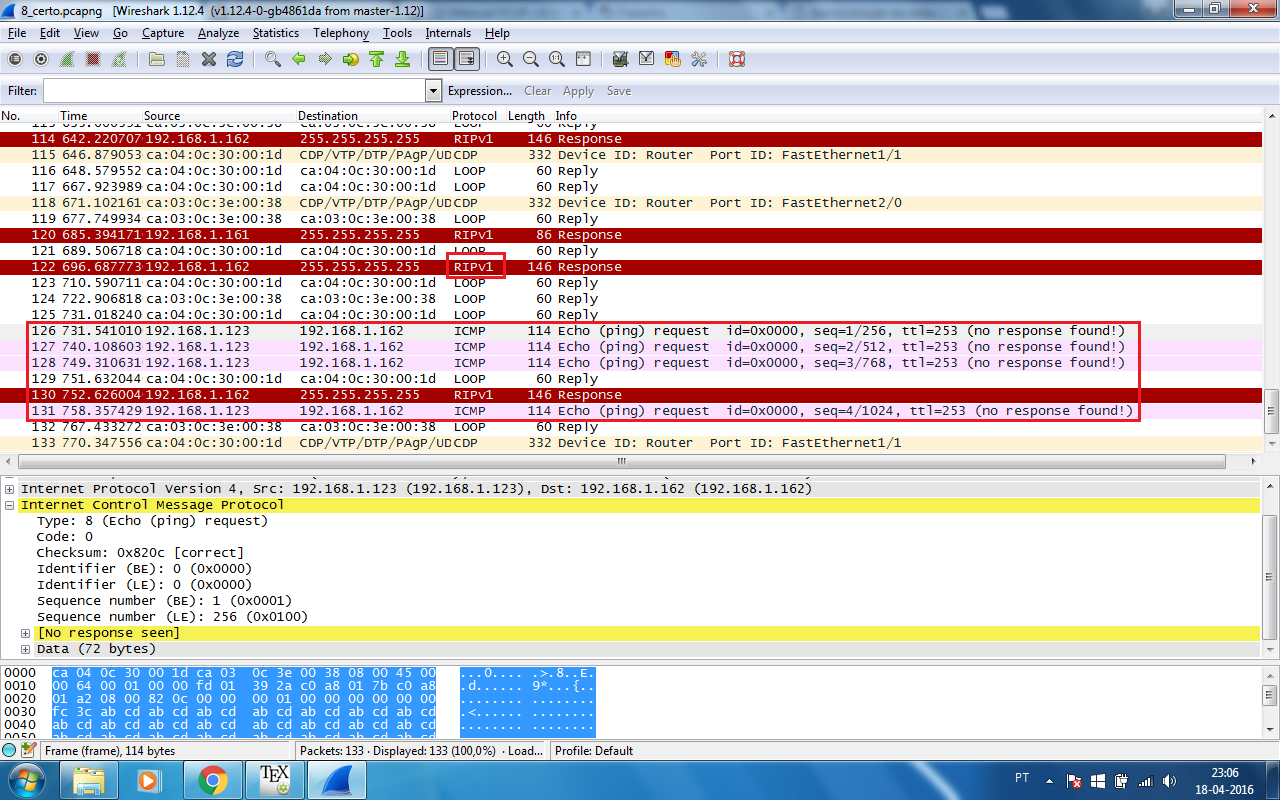
\includegraphics[width=1\textwidth, height=0.45\textheight]{8.png}
\label{fig:captura}
\caption{Captura na interface F1/1 de \textsf{R3}.}
\end{figure}
